\documentclass{gescons}

\genre {Entrevista}
\author{Ricardo Rezende}
\title{Ortoprincípios Norteadores da Invéxis}

\begin{document}
    \makeentrevistatitle
    \coverart{back/Ricardo_Rezende_Ortoprincipios}

\begin{center}
    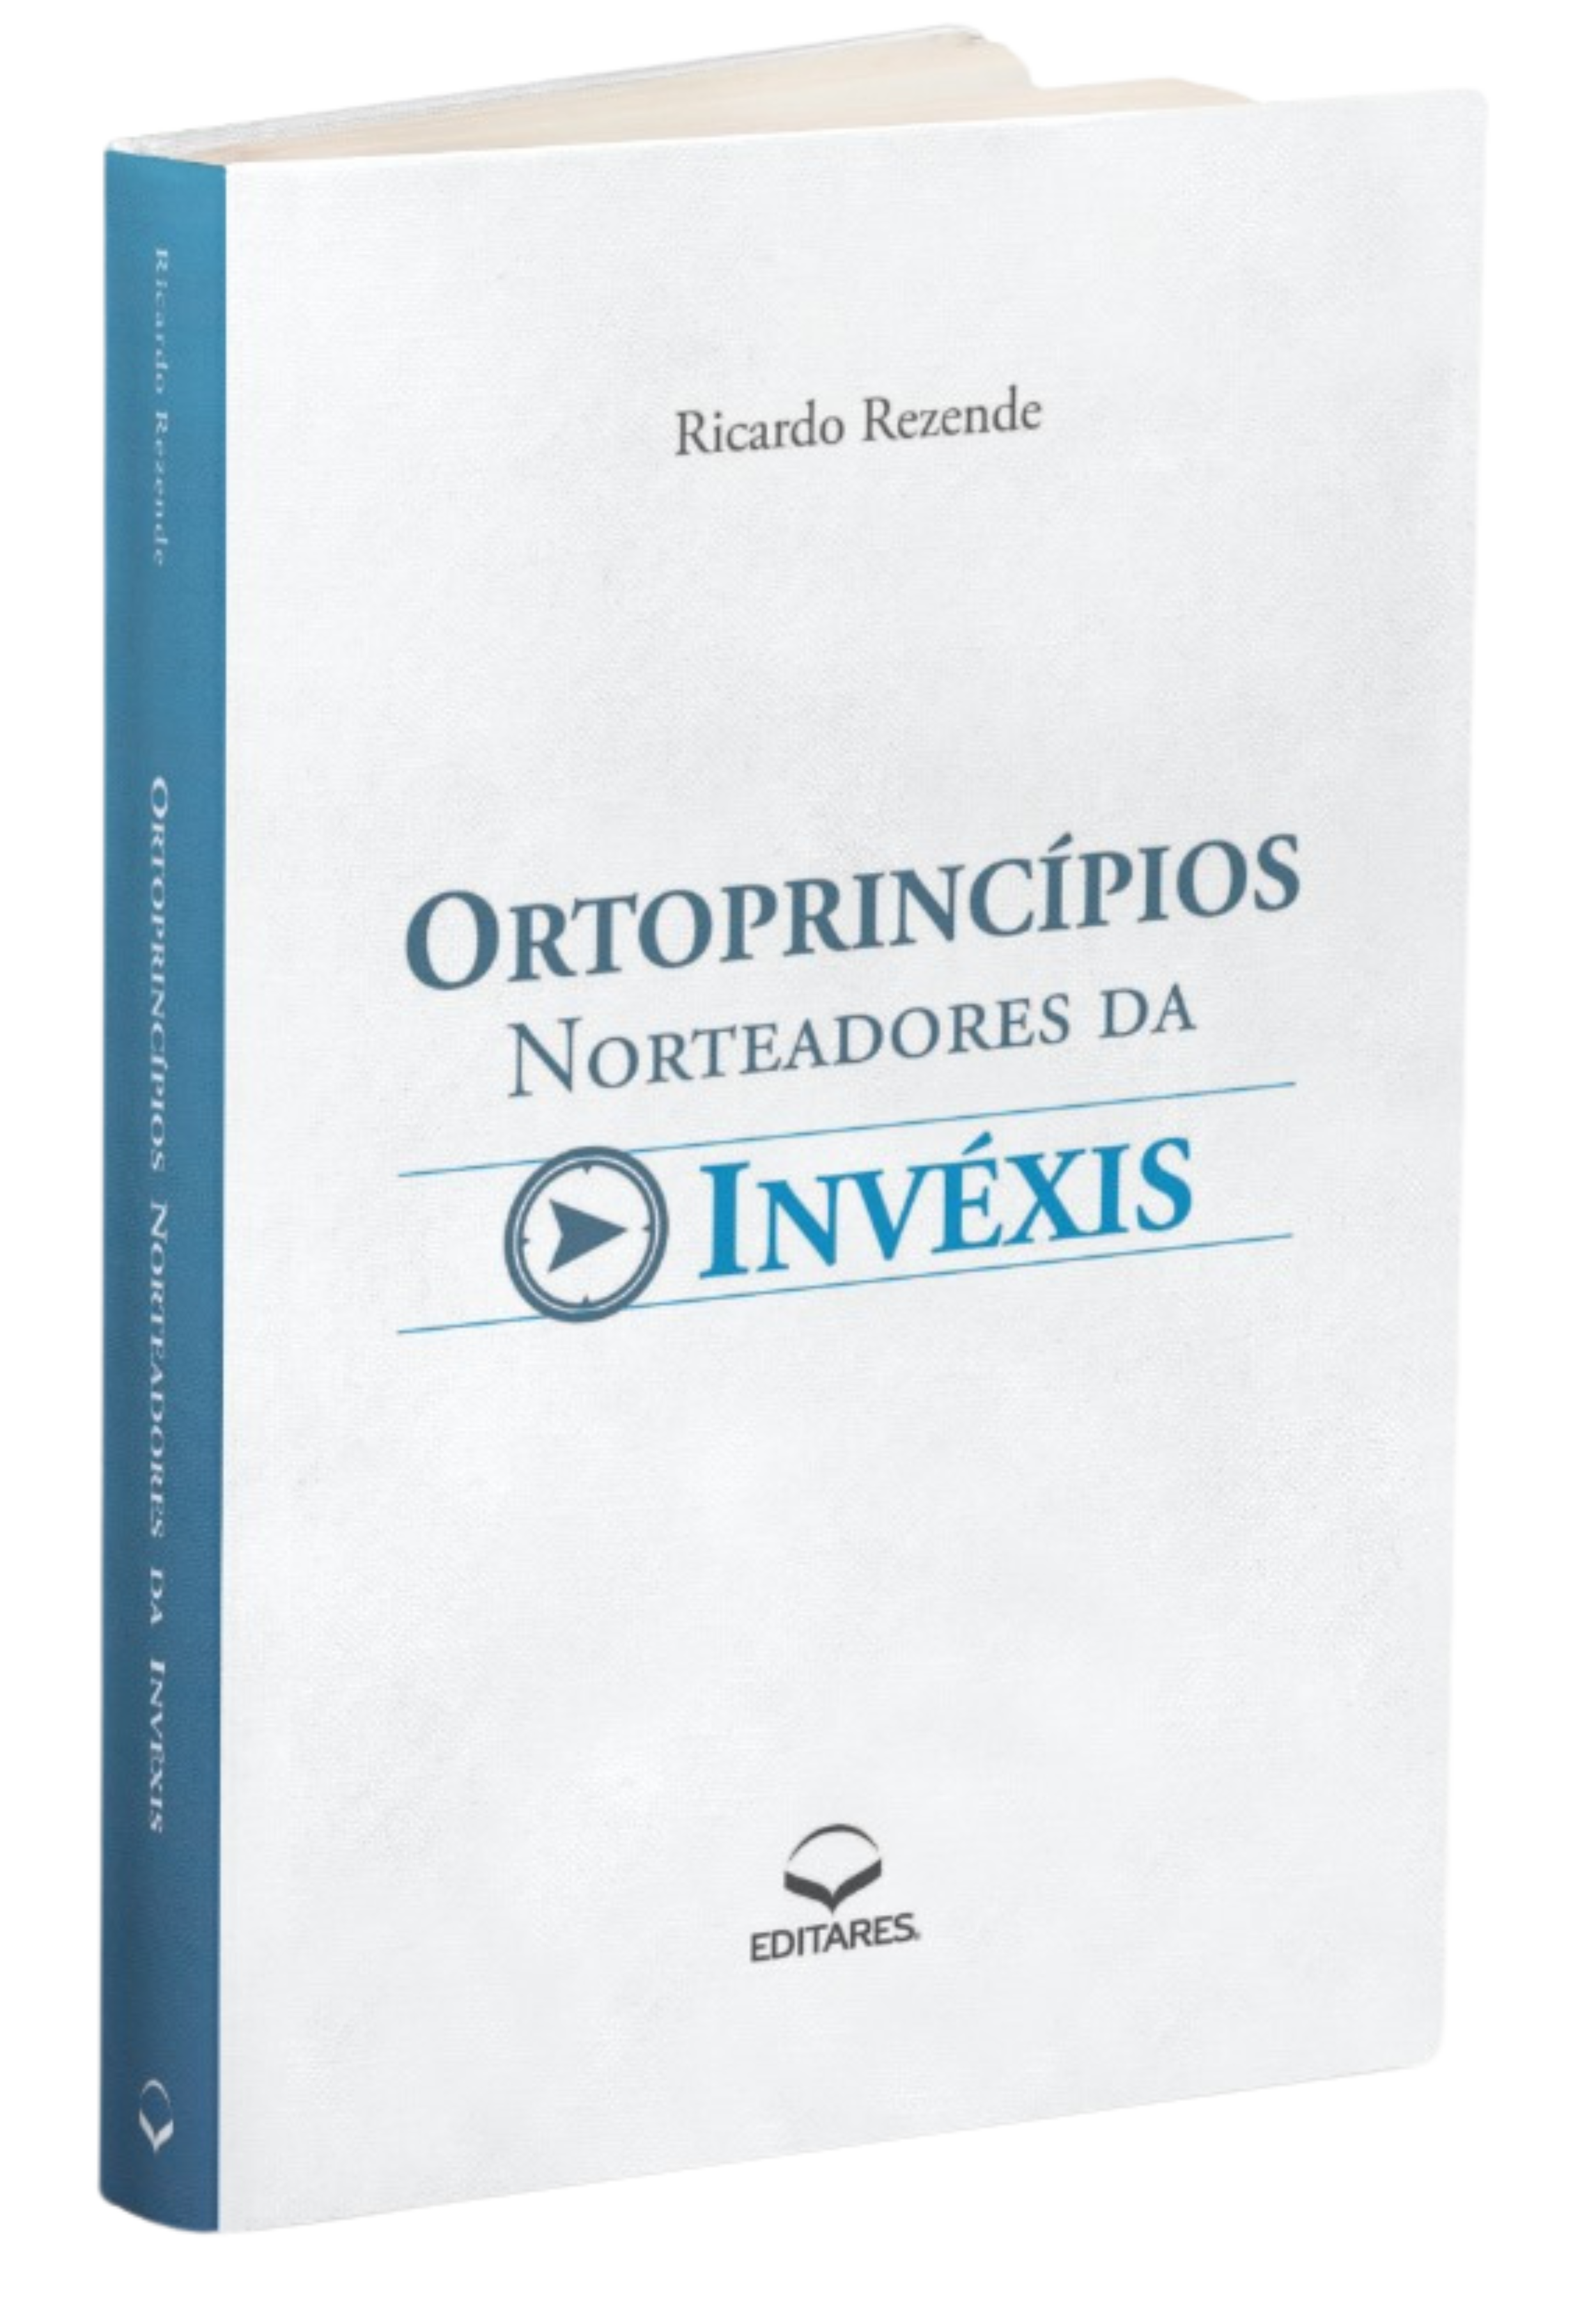
\includegraphics[width=7cm]{articles/entrevista/mockups/Ricardo-Rezende-Invexis.png}
\end{center}

    \begin{multicols}{2}


%\noindent\includegraphics[width=9cm, height=9cm]{example-image} 

\textbf{1. Qual foi a motivação para a escrita da obra? Por que a definição deste tema para publicação de um livro?}

Desde junho de 2022, este autor iniciou a escrita de verbetes a respeito de temas de Invexologia, incentivado pelo início dos trabalhos voluntários pessoais na Assinvéxis. Nesse período, houve imersão ou saturação intelectiva homeostática quanto aos conteúdos sobre inversão existencial, por meio da dedicação à verbetografia, resultando no estudo do tema \textit{holofilosofia da invéxis.}

Mais adiante para compreender melhor o assunto, iniciou-se mapeamento para identificar quais princípios cosmoéticos ou as \textit{condições evoluídas de se viver} poderiam compor a filosofia teática da inversão existencial. Para isso, realizou-se pesquisas em publicações conscienciológicas buscando localizar nos fundamentos ou nas bases teórico-práticas da Invexologia os ortoprincípios constituintes, de modo a estruturar a tese central da obra \textit{Ortoprincípios Norteadores da Invéxis.}

Portanto, essa obra advém da curiosidade pesquisística e determinação grafopensênica com o propósito de descortinar a filosofia teática da invéxis, sob 
o ângulo interdisciplinar de 5 especialidades: Principiologia, Experienciologia, Traforologia, Evoluciologia e Seriexologia.

\begin{pullquote}
``Essa obra advém da curiosidade pesquisística e determinação grafopensênica com o propósito de descortinar a filosofia teática da invéxis.''    
\end{pullquote}




\textbf{2. Qual o maior aprendizado com a escrita desta obra?}

A compreensão aprofundada da holofilosofia da invéxis, a expansão da paracognição invexológica e da lucidez invexometrológica pessoal.

\textbf{3. O que poderia dizer como incentivo para que mais pesquisadores invistam na publicação de obras conscienciológicas?}

O hábito da escrita conscienciológica com publicações seriadas resulta na ampliação dinâmica da hiperacuidade e na sustentação da conexão profícua com os amparadores extrafísicos e o holopensene homeostático da autoparaprocedência cursista, favorecendo o desenvolvimento intraconsciencial e da interassistencialidade tarística.


    
    
    \end{multicols}


\end{document}

